%%% Local Variables:
%%% mode: latex
%%% TeX-master: t
%%% End:


\documentclass[11pt,a4paper]{article}

\usepackage[french]{babel} \usepackage[T1]{fontenc} \usepackage[utf8]{inputenc}
\usepackage{graphicx}
\usepackage{amsmath,amssymb}
\usepackage{listings}
\usepackage{alltt}
\usepackage{array}

\title{TP -- Un émulateur Femto} \author{Grégoire Jadi \and Nicolas Grau}

\begin{document}
\maketitle

\tableofcontents


\section{Introduction}

Pour ce projet de l'année 2010/2011, il nous a été proposé d'étudier le fonctionnement d'un processeur
\textit{femto}.

Dans ce projet nous avons à réalisé le développement de deux programmes:

\begin{enumerate}
\item Un assembleur transformant en code machine un programme écrit en langage d’assemblage pour une
machine Femto .
\item Un émulateur exécutant le code machine produit par l’assembleur du point précédent de façon à
émuler une machine Femto.
\end{enumerate}

De plus, nous devrons faire en sorte que l'émulateur soit également capable de désassembler le code
produit.

Une interface semi graphique sera aussi à l'honneur afin de pouvoir visualiser le déroulement de
l'exécution d'un programme.

-- a deplacer a la conclusion ??
Cette étude nous permet aussi de comprendre de manière plus approfondie comment marche un
processeur, centre névralgique de tous les ordinateurs actuels.


\section{Dossier de Programmation}

Afin de gagner en clarté et efficacité nous avons décider de rédiger notre dossier en répondant aux
différents points proposés dans le sujet.

\subsection{Format utilisé}
\begin{quote}
Proposez un ou plusieurs formats pour la représentation des instructions (aide : on pourra utiliser
deux champs séparés pour le suffixe et l’opcode)
\end{quote}

Ici nous avons décidé d'utiliser un entier de 64 bits, composé comme suit:
\begin{itemize}
\item Une partie haute de 32 bits ou sera stocker la valeur du registre courant.
\item Une partie basse de 32 bits contenant le code de l'instruction.
\end{itemize}

Pour le codage de l'instruction nous avons choisis cette architecture:
\begin{itemize}
\item Les 8 premiers bits pour l'opcode, c'est à dire pour le choix de l'instruction du processeur
Femto.
\end{itemize}

\begin{itemize}
\item Les 3 bits suivants sont alloués pour le suffixe, car il n'y a que 5 suffixes différents.
\item Les bits restants sont divisés en trois, pour les registres rd, rs, rt. Ce qui nous donne 7
bits pour chaque registre.
\end{itemize}


\subsubsection*{Pourquoi avons nous choisis de donner plus de mémoire que nécessaire pour les instructions et les
registres ?}

Comme nous sommes visionnaires nous laissons de l'espace en vue d'une éventuelle évolution du
processeur femto le dotant soit de plus de mémoires, et donc plus de registres, soit d'un pannel
d'instructions plus large. Avec notre implémentation il n'y aura pas de problème pour
l'ajout d'un certain nombre d'instructions.

De plus les processeurs des machines actuelles travaillent généralement soit en 32 bits soit en
64 bits et ne peuvent manipuler des données plus petites. Ainsi, même si nous avions créé une structure
de données ayant exactement la taille minimale le compilateur \texttt{GCC} aligne les données pour faciliter
leurs manipulation. \footnote{on aurait pû interdire ce comportement à l'aide de l'instruction \texttt{\_\_attribute\_\_ ((packed))}
mais ce n'était pas très utile}

\subsubsection*{Pourquoi ne pas avoir fait la même chose pour le suffixe ?}

Il n'y a pas beaucoup de choix de suffixe possible, de ce fait nous avons considéré que tous le
suffixes possible était déjà présent. De ce fait nous n'avons pas alloué de l'espace supplémentaire
qui ne servirait pas à grand chose étant donné que cette partie n'est pas vraiment vouée à évolué.


\subsection{Programme en langage d'assemblage Femto}
\begin{quote}
Traduire en langage d’assemblage femto le programme ci-dessous :\end{quote}

\begin{alltt}
r0 = r0*r0 - 4*r1*r2; /* \begin{math} r0 = bˆ2 - 4ac \end{math} */
if (r0 > 0.0)
  r3 = 2.0; /* 2 solutions réelles */
else
  if (r0 == 0.0)
    r3 = 1.0; /* 1 solution réelle */
  else
    r3 = 0.0; /* aucune solution réelle */
\end{alltt}

Nous avons traduit le programme donné de la manière suivante:

\begin{alltt}
mulAL r4, r0, r0 // \begin{math} r1 =  r0^2 \end{math}
mulAL r5, r1, r2 // \begin{math} r5 = r1 * r2 \end{math}
loadAL r6, 4.0   // \begin{math} r4 = 4.0 \end{math}
mulAL r7, r5, r6 // \begin{math} r7 = 4 * r1 * r2 \end{math}
subAL r0, r4, r7 // \begin{math} r0 = r0 * r0 - 4 * r1 * r2 \end{math}

loadAL r3, 0.0   // par défaut il n'y a pas de solution

loadAL r1, 0.0
cmpAL r1, r0     // on compare r0 avec 0
loadLT r3, 2.0   // si \begin{math} r3 > 0 \end{math} alors \begin{math} r3 = 2 \end{math}
loadEQ r3, 1.0   // si \begin{math} r3 == 0 \end{math} alors \begin{math} r3 = 1 \end{math}

\end{alltt}

\begin{quote}
Proposer au moins deux programmes (langage d’assemblage et code machine) utilisant les possibilités
de la machine femto
\end{quote}

Nous avons proposé trois programmes simples:

\subsubsection*{Un programme calculant une fonction de type $ ax^{2} + bx + c $ avec demande des paramètres}

\begin{alltt}
// demande des différents coeff
readAL r0 //lecture de a
readAL r1 //lecture de b
readAL r2 //lecture de c

readAL r4 // demande de la valeur de x

// calcul
mulAL r5,r4,r4 // \begin{math} x^2 \end{math}
mulAL r6,r5,r0 // \begin{math} ax^2 \end{math}
mulAL r7,r1,r4 // \begin{math} bx \end{math}

addAL r8,r6,r7 // \begin{math} ax^2 + bx = d \end{math}
addAL r9,r8,r2 // \begin{math} d + c = ret \end{math}

//affichage
printAL r9 //affichage résultat
\end{alltt}


\subsubsection*{Un programme calculant la racine carrée d'un nombre}

\begin{alltt}
// fonction qui calcul la racine carré d'un nombre

readAL r0 //demande du nombre

//si ce nombre est négatif alors on arrête le programme
loadAL r1, 0.0
cmpAL r0, r1
stopLT

//si ce nombre est égal à 0 on renvoie 0 et on arrête le programme
printEQ r0
stopEQ

//si ce nombre est supérieur à 0 on renvoie la racine
cmpAL r1, r0
powLT r2,r0, 0.5
printLT r2
\end{alltt}

\subsubsection*{Suite de Fibonacci}

\begin{alltt}
readAL r15 // lecture de n

// initialisation des registres
loadAL r0, 0.0
loadAL r1, 1.0

// si n < 1 on quitte le programme apres avoir affiche le resultat
loadAL r5, 1.0
cmpAL r15, r5
printLT r0
stopLT

// debut de la boucle
addAL r2, r1, r0
moveAL r0, r1
moveAL r1, r2
subAL r15, r15, r5

// si n <= 1 on sort
cmpAL r5, r15
bLT -5

// on affiche le resultat et on quitte le programme
printAL r2
stopAL
\end{alltt}

\subsection{L'émulateur Femto}

\begin{quote}
Ecrire un émulateur pour la machine femto. On précisera soigneusement les hypothèses de travail
(taille de la mémoire, taille d’une case de la mémoire, . . .) dans le dossier. L’émulateur devra
lire le programme à émuler dans un fichier sous forme de code machine
\end{quote}

On ne fait aucune supposition sur la taille de la mémoire de la machine cible, c'est à dire de la
machine sur laquelle l'émulateur Femto, et afin de garantir le bon fonctionnement\footnote{Dans une
certaine mesure, on n'évitera pas un rollback sur le pointeur d'instruction si le nombre
d'instructions du programme chargé n'est pas représentable sur un entier (dont la taille peut varier
selon la machine)} du programme on utilise le fichier d'en-tête standart (C99) \texttt{stdint} qui
nous permet d'utiliser les types suivants:
\begin{description}
\item[uint8\_t] qui fait 8 bits
\item[uint32\_t] qui fait 32 bits
\item[uint64\_t] qui fait 64 bits
\end{description}

Ainsi, une instruction complète -- opcode + suffixe + registres + valeur -- sera représentée sur un
\texttt{uint64\_t}.

Nous avons choisi que les instructions soit représentée en format décimal et non pas en binaire «
pur » ce qui qui nous permet de éditer les fichiers à l'aide d'un simple éditeur de texte.

\subsubsection*{Représentation en mémoire}

Le programme va lire le fichier ligne par ligne et stocker toutes les instructions dans une
structure de données que l'on appelera par la suite \texttt{contexte}. Ce nom lui correspond bien,
puisqu'elle contient non seulement un tableau contenant l'ensemble des instructions du programme
courant, mais aussi le nombre d'instruction dudit tableau et surtout la valeur du pointeur
d'instruction ainsi que les drapeaux (qui correspondent au résultat de la dernière
comparaison). C'est donc bien l'état du programme en cours d'émulation.

\subsubsection*{Déroulement de l'émulation}

L'exécution du programme ainsi chargé est désormais relativement simple, on parcourt le tableau
d'instruction en utilisant le pointeur d'instruction comme repère dans celui-ci. Par conséquent,
si jamais une instruction de branchement est exécutée il lui suffit de modifier la valeur du pointeur
d'instruction pour modifier le flux du programme.

Lorsque l'on arrive à une instruction, on la décompose en séparant les différents champs et en les
interprétant correctement. Ainsi une instruction ne sera exécutée que si le suffixe le permet par rapport
à l'état actuel des drapeaux.

Ensuite le pointeur d'instruction est incrémenté et on recommence.

\subsection{Désassemblage d'un programme Femto}

\begin{quote}
Modifier l’émulateur pour permettre le désassemblage du code lu (passage du code machine au code
en langage d’assemblage) et son affichage à l’écran
\end{quote}

Le désassemblage d'un programme est très similaire à l'exécution dudit programme.

En effet, on initialise le contexte de la même manière, simplement on ne va pas suivre le flot
habituel du programme, on va simplement afficher les instructions les unes après les autres.

\subsection{Exécution pas-à-pas}

\begin{quote}
Modifier l’émulateur pour permettre l’exécution pas-à-pas du code lu
\end{quote}

L'exécution en mode pas-à-pas est également très simple une fois l'émulateur et le désassemblage
fonctionnel.

En effet, il suffit d'afficher l'instruction courante avant de l'exécuter et d'attendre que
l'utilisateur appuie sur la toucher \texttt{entrée}.

Comme nous avions modularisé notre code pour le désassemblage, il nous a suffit de reprendre la
fonction affichange l'instruction courante désassemblée et intégrer l'attente de l'utilisateur au
code de l'émulateur.

\subsection{Réalisation d'un assembleur}

Afin de faciliter la réalisation des tests nous avons codé un petit assembleur traduisant le code
assembleur femto en un fichier correspondant au format de notre émulateur Femto.

Pour cela, on utilise les outils d'analyse gramaticale bien connus que sont Bison et Flex.

L'assembleur gère les commentaires de la forme \texttt{\/\/}. Cependant, il faut bien utiliser des
nombres flottants pour les instructions \texttt{load}, \texttt{pow} et des entier pour l'instruction
\texttt{b}.

Dans le cas où le fichier serait mal formé, on affiche juste le message "syntax error" sans plus
d'explication.

\subsection{Réalisation d'une interface graphique}

\begin{quote}
[Optionnel] Utiliser les fichiers GUI disponibles sur madoc pour ecrire une interface semi-graphique
a l’émulateur permettant d’afficher simultanéement le contenu de la mémoire et des registres lors de
l’exécution du programme pas-à-pas.
\end{quote}

Pour réaliser une pseudo-interface graphique, nous utilisons les quelques fonctions fournies qui fournissent
une petite API à la bibliothèques \textbf{NCurses}.

L'interface est assez sommaire par manque de temps.

Le programme est exécuté en mode pas-à-pas et le contenu des registres est affiché après chaque
instruction dans un cadre à part.

On passe à l'instruction suivante en appuyant sur n'importe quel touche, lorsqu'une saise est
requise un message apparait dans un cadre et l'on attend que l'utilisateur entre un nombre (pas de
gestion d'erreurs).

Lors d'un affichage, le résutat apparait dans le cadre approprié.

Voici un apperçu de l'interface:


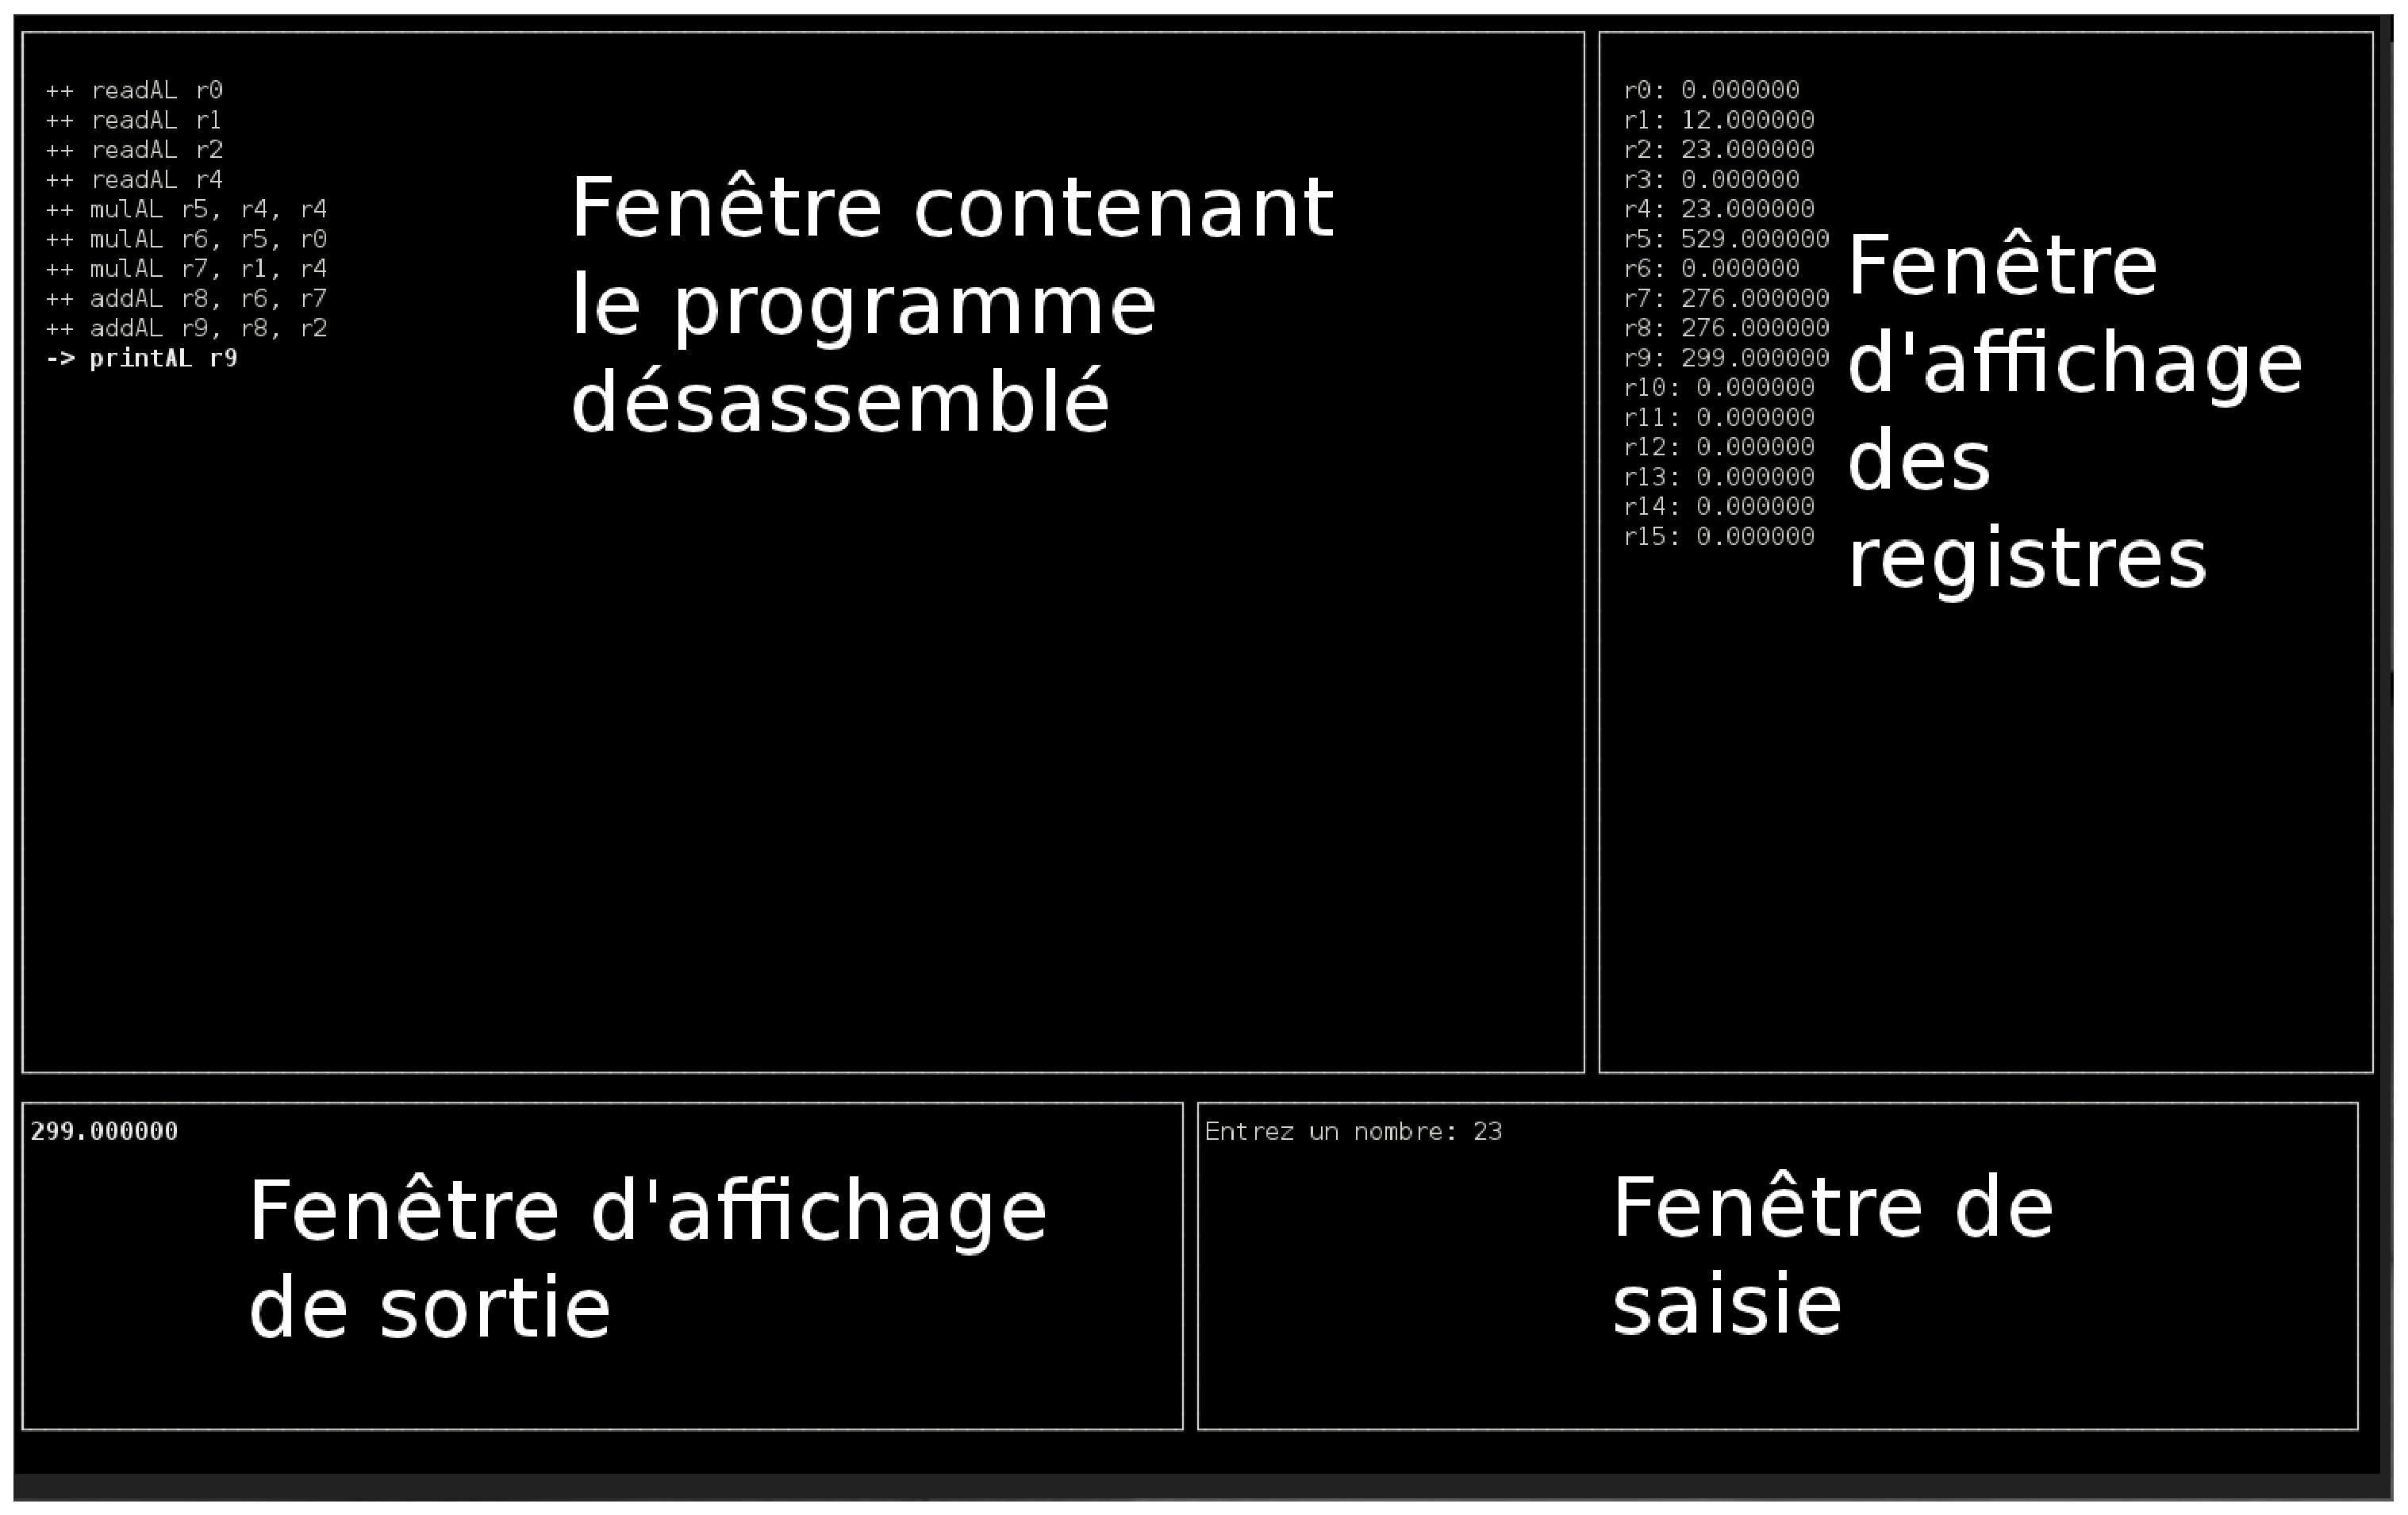
\includegraphics[scale = 0.3]{./fgui.eps}


\end{document}
